\documentclass{standalone}
\usepackage{tikz,tkz-euclide}
\usepackage{ctex}
\setCJKmainfont{Noto Serif CJK SC}
\usepackage{mhchem,siunitx}
\begin{document}
\small
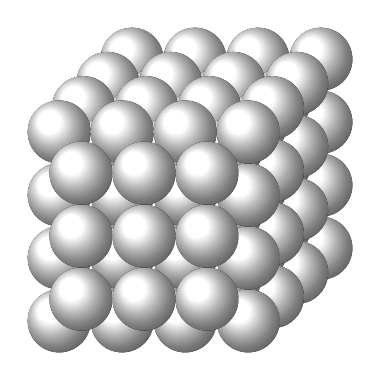
\begin{tikzpicture}[>=stealth,scale=1.6,inner sep=2pt]
  \foreach \z in {0,1,2,3}
  {
    \foreach \x in {-1.5,-0.5,0.5,1.5}
    {
      \foreach \y in {-1.5,-0.5,0.5,1.5}
      \fill[ball color=white](0.5*\x,0.5*\y,0.5*\z)circle(0.25);
    }
    \foreach \x in {-1,0,1} 
    {
      \foreach \y in {-1,0,1}
      \fill[ball color=white](0.5*\x,0.5*\y,0.5*\z+0.2)circle(0.25);
    }
  }
\end{tikzpicture}
\end{document}